\documentclass[border=10pt]{standalone}
\usepackage{xcolor}
\usepackage{pgfplots}
\usepackage{tikz}
\begin{document}
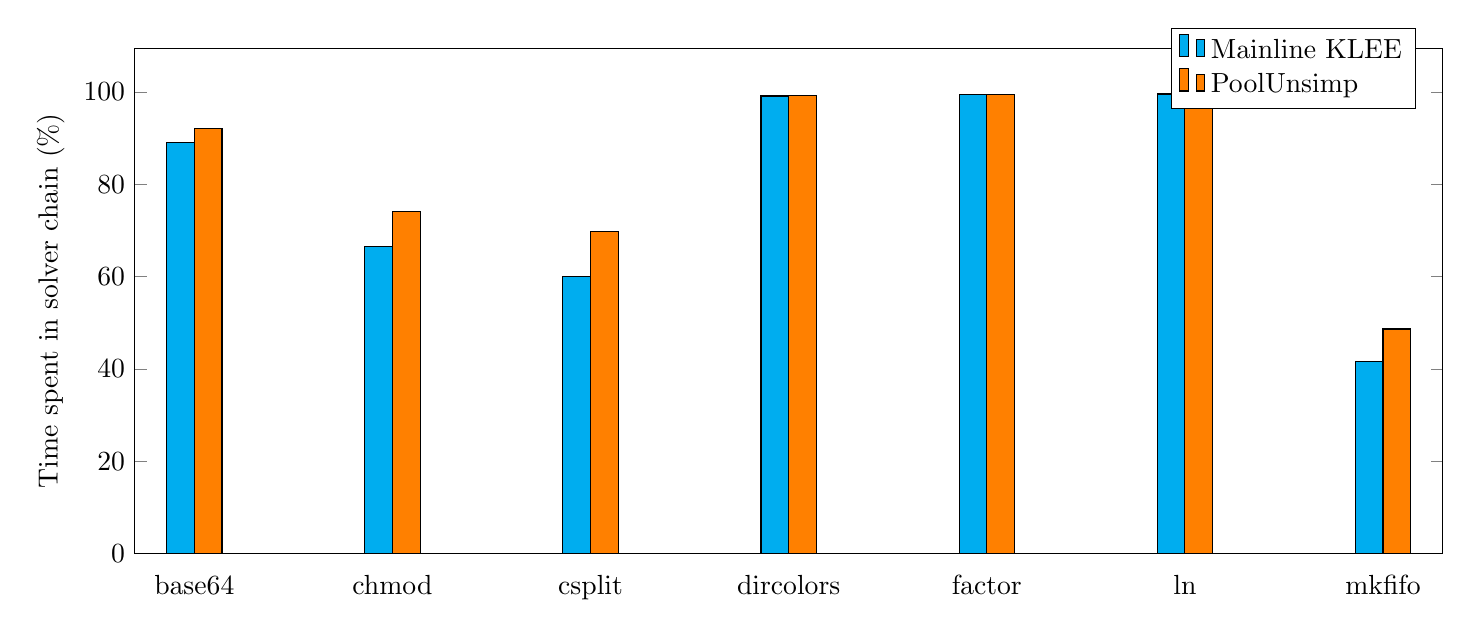
\begin{tikzpicture}
    \begin{axis}[
        width  = 1.5 * \textwidth,
        height = 8cm,
        major x tick style = transparent,
        % tickwidth=10,
        ybar=0,
        bar width=10pt,
        % ymajorgrids = true,
        ylabel = {Time spent in solver chain (\%)},
        symbolic x coords={base64,chmod,csplit,dircolors,factor,ln,mkfifo},
        xtick = data,
        scaled y ticks = false,
        enlarge x limits=0.05,
        ymin=0,
        legend cell align=left,
        legend style={
                at={(0.98,0.88)},
                anchor=south east,
                % column sep=1ex
        }
    ]
        \addplot[style={cyan,fill=cyan,mark=none}, draw=black]
	coordinates {(base64,89.03) (chmod,66.41) (csplit,60.08) (dircolors,99.10) (factor,99.41) (ln,99.53) (mkfifo,41.62)};
\addplot[style={orange,fill=orange,mark=none}, draw=black]
	coordinates {(base64,92.15) (chmod,74.17) (csplit,69.81) (dircolors,99.22) (factor,99.49) (ln,99.22) (mkfifo,48.63)};

        \legend{Mainline KLEE,PoolUnsimp}
    \end{axis}
\end{tikzpicture}
\end{document}
